\begin{figure}[!t]
\centering
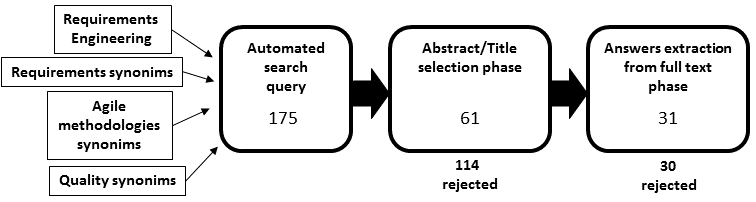
\includegraphics[scale=0.75]{images/1_study_methodology}
\caption{Summary of our search process}
\label{fig:study_methodology}
\end{figure}

\section{Results}

The automated search query have obtained 175 studies. From those, 61 were chosen to a full reading and 31 have answered one or another research questions. This whole process is summarized in Figure \ref{fig:study_methodology} and the 31 accepted papers are shown in Table \ref{table:accepted_papers}.

\begin{table}[!t]
\centering
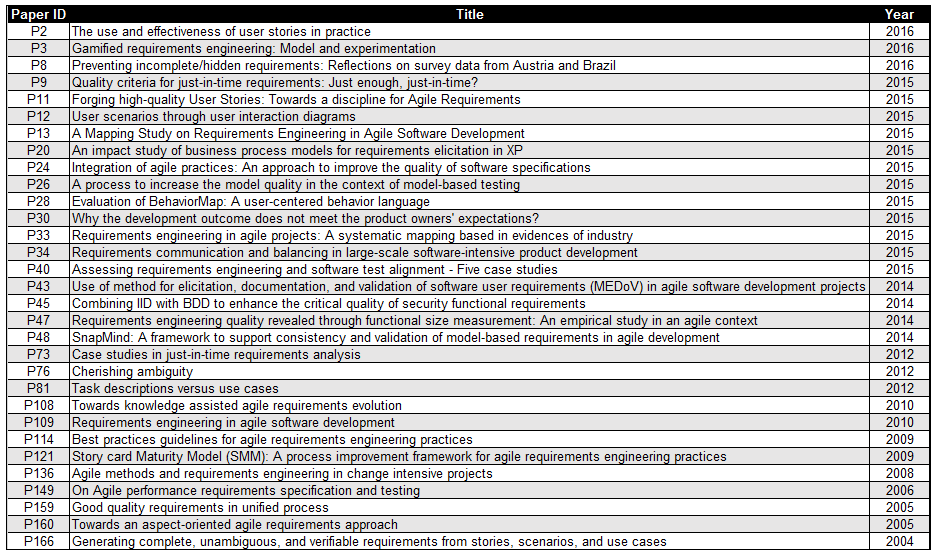
\includegraphics[scale=0.63]{images/PaperID_reference}
\caption{Accepted papers identification}
\label{table:accepted_papers}
\end{table}

\begin{figure}[!b]
\centering
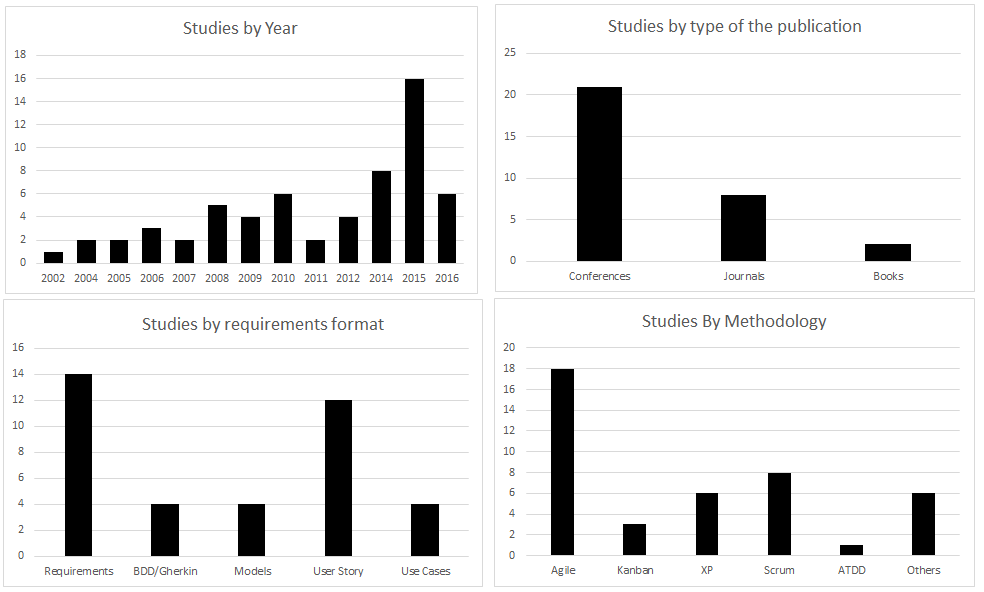
\includegraphics[scale=0.6]{images/2_charts}
\caption{Studies overview}
\label{fig:charts}
\end{figure}

\subsection{Studies Overview}

Given those studies that have answered our research questions, most of them (21 from 31) were published on conferences or workshops, while a few (8 from 31) were published on journals, and the rest of them (2 studies) were found on books chapters. Also, by looking at the publication year from the obtained results, one can see that many studies from the last 4 years were obtained. 

When we look at what agile methodology each study follows, we can see that the most of them talk about agile in a broad and generic way, without mentioning any specific methodology. This approach is the same one when talking about format of requirements. Even with the popularity of the User Story format from many studies uses "agile requirements" as the focus of their work. Many studies have tried to compare one or other methodology or map one requirement format on another, so the were counted twice (or more) on the detailed charts in Figure \ref{fig:charts}.

\subsection{Concept of Requirements Quality on Agile Development}

The answers to \textbf{RQ1} were related to the concept of requirements quality on agile development and can be found summarized in Figure \ref{fig:answers_rq1}. However, the majority of the studies (51\%) did not answer this question directly, as they faced quality of requirements as a list of aspects. Agile RE documentation matching those aspects are considered to be good ones. In contrast, almost a third of the studies (29\%) do not focus on the requirements documentations to decide what a good requirement is. Instead, they understand that good requirements is when customer's needs and expectations are met. A small parcel of studies (10\%) understand that the definition of quality is a checklist that requirements shall attend to in order to be considered ready to be developed. Another small percentage of studies (10\%) understand that the lack of problems on requirements is enough of a guarantee of quality.

\begin{figure}[!h]
\centering
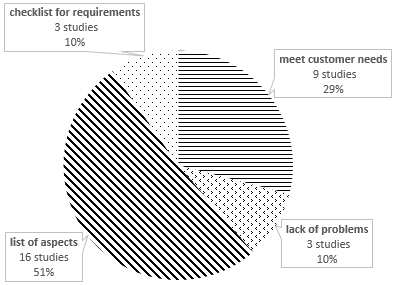
\includegraphics[scale=1]{images/3_answers_rq1}
\caption{Summary of answers to RQ1}
\label{fig:answers_rq1}
\end{figure}

\begin{table}[!t]
\centering
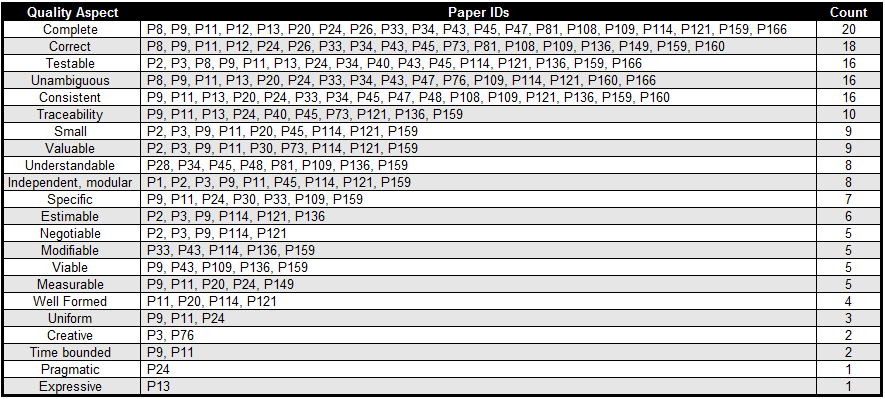
\includegraphics[scale=0.65]{images/QualityAspect_ListOfPapers}
\caption{List of aspects on each accepted paper}
\label{table:aspects_per_paper}
\end{table}

\subsection{Aspects Used to Evaluate Requirements Quality on Agile Development}

The research question \textbf{RQ2} seeks to understand what aspects were used on agile methodologies to evaluate the quality of requirements. The aspects obtained on the accepted papers are shown on Table \ref{table:aspects_per_paper}, along with the papers identification codes that referenced that characteristic. The last column, counting the number of papers referencing the rows aspect, shows us that the traditional aspects found on \cite{Babok_2015} and \cite{Babok_2009} are still relevant, as we see that characteristics such as completeness, correctness, testability, lack of ambiguity, and consistency are the top ones mentioned.

However, alternative techniques like SMART and INVEST \cite{SMART_INVEST_2013} have been present as well, specially to complement attributes that are not covered by traditional references, such as the size of requirements and the importance of them to the client. The concern with requirements traceability highlighted on \cite{Inayat_2015} is also one criteria that appears on some publications (10 out of 31).

Other characteristics of requirements, such as expressivity, uniformity, and language clarity are not taken into account that often. It may indicate that the writing of the requirements description is not a concern on agile requirements, due to the practices found on \cite{Inayat_2015} that focus on face-to-face communication to define details. 